The grasping system proposed, shown in Figure \ref{fig:systemArchitecture}, consists of a learned generative model and an evaluative model. The generative model is a method that generates a number of candidate grasps given a point cloud, as explained in the previous section. An evaluative model is paired with a generative model in order to estimate a probability of success for each candidate grasp. EM1 and EM3 are VGG-16 based visual models, while EM2 is a modified ResNet-50 architecture. All evaluative models process the visual data and hand trajectory parameters in two separate pathways, and combine them to feed into a third processing block to produce the final success probability. The generative models GM1 and GM2, and the evaluative models EM1-3 are interchangeable, creating 6 generative-evaluative model pairs. 

The generative model produces 1000 grasps in 15 seconds on a 2x Intel Xeon E5-2650 v2 Eight Core 2.6GHz. There is, however, no estimate of the probability of grasp success. This the purpose of the evaluative model. Deep networks have been shown to learn good evaluative models of grasp success for two finger grippers and for dexterous hands (Barrett, Allegro) performing power grasps.  

%In this section, our evaluative deep network architecture is described. In the following section, the simulation used to generate the training data is detailed.
%First, the generative model largely ignores global information about the object; relying instead on global information about the hand shape, and local information about finger-object contacts. To predict grasp success probability we need a learner that somehow takes into account global information, such as global shape, mass, mass distribution, friction coefficients, deformability, etcetera. The difficulty with this is that, given a single depth image, the learner does not have direct access to these. Thus, they cannot be estimated, but all that can be learned is the association Second, the 

%It is time-consuming and expensive to collect real grasp data with using robotic arms with dexterous hands. Unlike gripper + arm combinations which require relatively less supervision \cite{Levine1}, dexterous hands can be much more fragile due to their complexity. Advances in physics simulators have made it possible to re-create robotic experiment setups in simulation. We created a simulated experimental setup in order evaluate grasp, which allowed us to collect as much data as needed in a short period of time with no supervision.

We now present the formulation of an evaluative network $f(I_t, h_t)$, where $I^t$ is a colourized depth image of the object, and $h_t = (h_{tw}, h_{tc})$ gives the sequence of wrist poses and hand configurations for a grasp, expressed in the camera frame. The network outputs a grasp success probability for image-grasp pair $I_t$, $h_t$. Section~\ref{section:simulation} gives details of the simulation used to generate the training data.
% The purpose of the network is to learn the relationship between the point cloud, given as a colorized depth image, and grasp (hand shape) parameters which encode the configuration of the hand with respect to the camera frame. This is a complex task, as the kinematic model of the hand is unknown to the network, and it has to consider each grasp as a black box: The network knows the inputs that configure the hand, including the joint positions, and only has access to the outcome in the form of success/failure. 
% Talk more about the architecture
An evaluative model relies on two inputs: the depth image of the scene, and grasp trajectory parameters. In order to obtain the visual input, pre-processing segments the table plane from the object point cloud of the object. The segmented $640 \times 480$ depth image $I_{t}^{depth}$ is cropped to a window of $460 \times 460$, located in the image centre. Then, it is down-sampled to $224 \times 224$. The colourization creates a $224 \times 224$ 3-channel image $I_t$. The channels  are the mean curvature, the Gaussian curvature, and the depth. The second input, the hand trajectory, $h_t$ comprises 10 way-points, each of 28 dimensions (20 for the finger joint angles, 1 for the grasp type, and 7 for the wrist pose), giving 280 dimensions. %The formula of mean curvature is $h = {gr}_{xx} + {gr}_{yy}$, where ${gr}_{xx}$ is the second gradient in horizontal direction in a $1 \times 3$ window, and ${gr}_{yy}$ is its vertical counterpart. Similarly, Gaussian curvature $k = {gr}_{xx} \times {gr}_{yy} - ({gr}_{xy})^2$.
% The final three layers are fine-tuned, while the first 13 layers are frozen.
% For visual processing, we use a deep network pre-trained on ImageNet. 
%This is transformed to 1024 using a single layer. This and the output of the final layer of the visual block are element-wise added. Then there are four fully connected layers each comprising 1024 RELU nodes. The output is a grasp success/failure probability, encoded by two softmax nodes.  We train using the cross-entropy loss function:
\begin{equation}
H_{y'}(y) := - \sum_{i} ({y_i' \log(y_i) + (1-y_i') \log (1-y_i)})
\label{equation:crossentropy}
\end{equation}
where $y_i'$ is the ground truth success (1) or failure (0); $y_i = f(I_i, h_i)$ is the predicted grasp success of grasp trajectory $h_i$, and $I_i$ is the associated colourized depth image of grasp $h_i$.
\begin{figure}
\begin{center}
  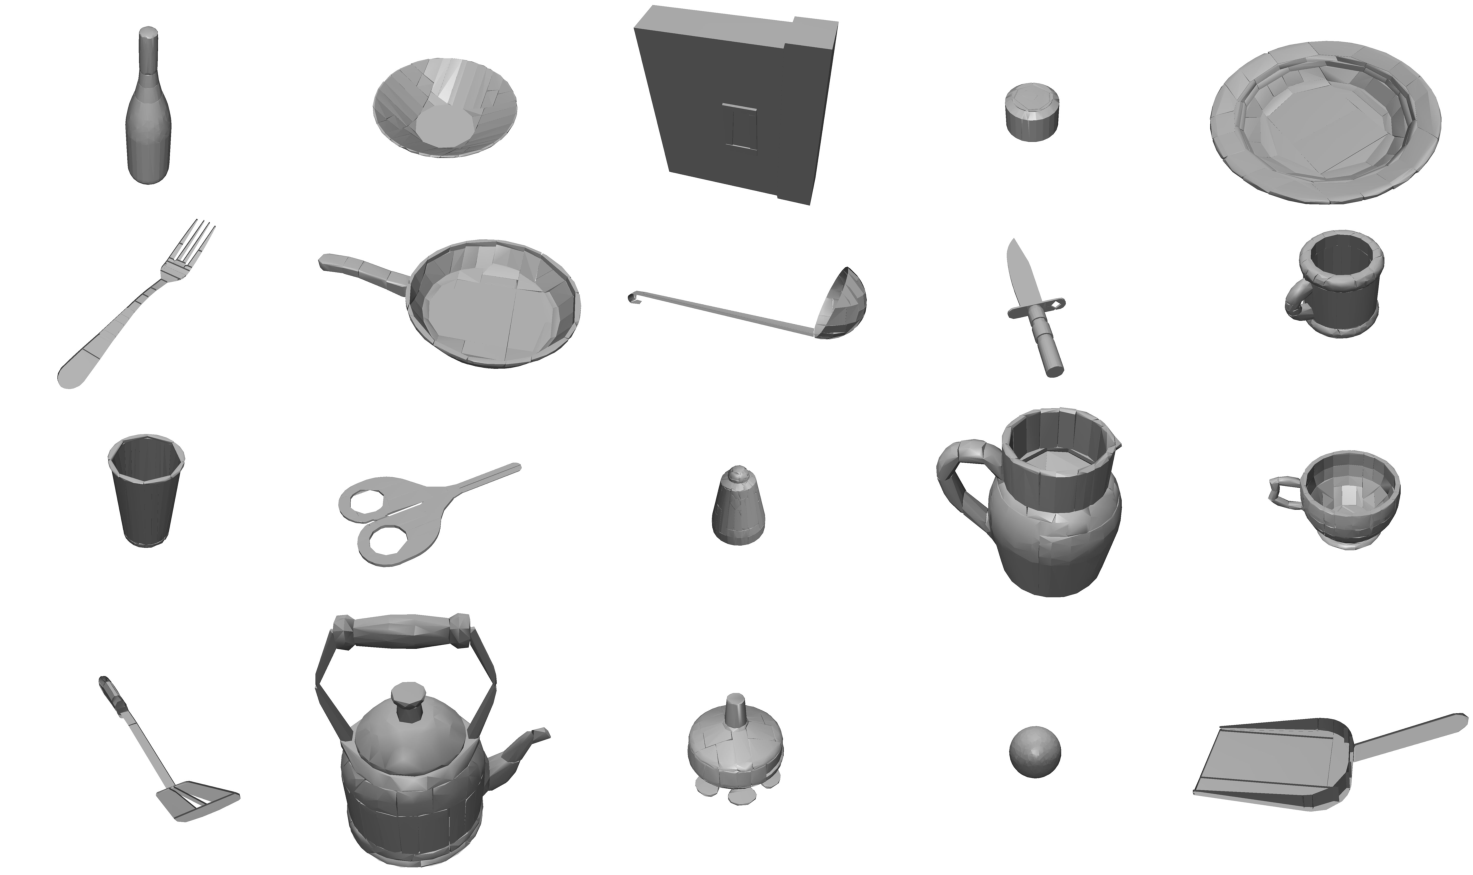
\includegraphics[width=0.9\linewidth]{images/allObjects-small.pdf}
  \end{center}
  \caption{Sample objects from all classes in the 3D model dataset.}
  \label{fig:allObjects}
\end{figure}
We trained our network on a data set of simulated grasps. We now describe the simulation used to generate a realistic training set. % o 7000 distinct scenes, where each scene contains a random instantiation of one of the objects in the dataset with varying rigid body transformations applied, as well as friction and weight changes. The network was tested on 80000 grasps on 1200 scenes of unseen objects, as well as real robot experiments, as explained in Section \ref{section:experiments}. In order to make a direct comparison with Kopicki et al. \cite{kopicki2015ijrr}, we pick top grasps based on both the original ranking, as explained in Section \ref{section:generative}, and according to the predicted success probabilities by the network. 

%We opted to use a grasp success prediction network due to the fact that the grasp generator function, explained in the previous chapter, provides alternatives of most intuitive types of grasps. A logical extension of this work would be to pair our learning algorithm with a grasp generator network, which we consider as future work.

%Overall network architecture. VGG summary. Description of new layers. Representation of hand parameters, frames of reference, camera image conversion for VGG, trajectory of wrist and fingers.